\documentclass[12pt,a4paper]{article}
\usepackage[utf8]{inputenc}
\usepackage[german]{babel}
\usepackage[T1]{fontenc}
\usepackage{amsmath}
\usepackage{amsfonts}
\usepackage{amssymb}
\usepackage{graphicx}
\usepackage[left=2.5cm,right=2.5cm,top=2cm,bottom=2cm]{geometry}
\usepackage{float}
\author{Gruppe C14 \\ Julián Häck, Martin Koytek, Lars Wenning, Erik Zimmermann}
\begin{document}
\section{Aufnahme eines Frequenzspektrums}
\subsection{Versuchsbeschreibung}
Bei Grundschwingungen (1. Harmonische) befinden sich die Knoten an den Saiten-Enden. Neben der Grundschwingung bilden sich aber auch weitere sogenannte Oberschwingungen aus, die an den Enden ebenfalls Knoten bilden. Für die Wellenlängen dieser so genannten  n-ten Harmonischen gilt:
\begin{equation}
\lambda_n=	\frac{2L}{n}
\end{equation}
Für n=1 ergibt sich die Grundschwingung für n = 2 die 1. Oberschwingung für n = 3 die 2. Oberschwingung und so weiter.
\newline
\begin{figure}[H]
\centering
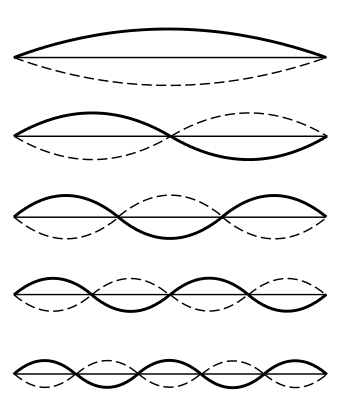
\includegraphics[scale=1]{Bilder/Harmonische.png}
\caption{Stehende Welle und deren Harmonische bis n = 5.}
\end{figure}

Schlägt man die Saite im Abstand $d=\frac{L}{n}$ an, fehlen die n-te Harmonische und ihre Vielfachen, da sich dort kein Knoten bilden kann.

In diesem Versuch sollte das Frequenzspektrum der D-Saite einer Gitarre, die an verschiedenen Abständen angeschlagen wurde auf das oben beschriebene Verhalten untersucht werden.

\newpage
\subsection{Versuchsaufbau und Durchführung}
Der Aufbau ist derselbe wie in den anderen Versuchen zur Gitarre. 

\begin{table}[H]\centering
\caption{Messparameter für Aufnahme des Frequenzspektrums der D-Saite.}
\begin{tabular}{c|c}
Parameter & Einstellungen \\ 
\hline
Messintervall & 100 $\mu s$ \\ 
Anzahl Messwerte & 16000 \\ 
Messdauer & 1.6s \\ 
Trigger & 0.3V \\ 
\end{tabular}
\end{table}

Als Erstes wurde die D-Saite in der Mitte angeschlagen.
\begin{figure}[H]
\centering
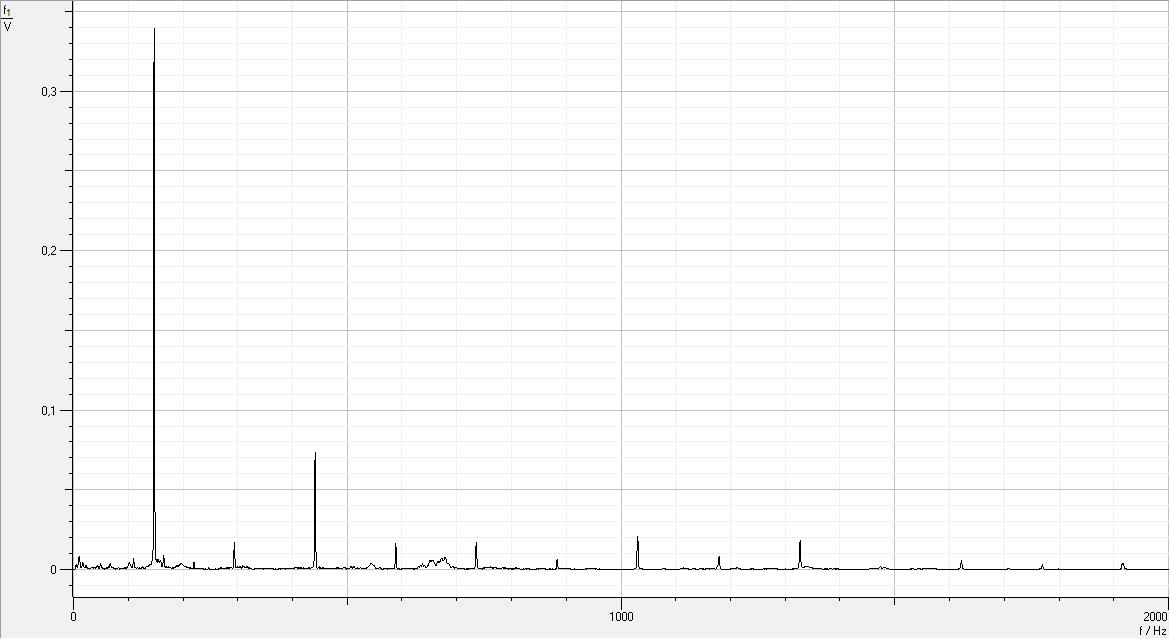
\includegraphics[scale=0.45]{Bilder/Spektrum_Mitte.png}
\caption{Grundfrequenz von 147,03 Hz ist deutlich erkennbar. Nur jede zweite Schwingung ist ausgeprägt.}
\end{figure}

Zum Vergleich wurde die Saite sehr weit oben am Hals angeschlagen.
\begin{figure}[H]
\centering
\includegraphics[scale=0.45]{Bilder/Spektrum_oben.png}
\caption{Die Amplituden fallen bis zur 6. Harmonischen stetig ab.}
\end{figure}

\subsection{Fazit}
Wie in den gezeigten Abbildungen zu sehen ist, konnten wir die Theorie, dass die n-ten Harmonischen fehlen, wenn man die Saite an einem Abstand von $d=\frac{L}{n}$ anschlägt, bestätigen.

\end{document}